%%%%%%%%%%%%%%%%%%%% manuscript.tex %%%%%%%%%%%%%%%%%%%%%%%%%%%%%%%%%%%
%
% Springer proceedings template (svproc class)
% Content: CARLA-MAMBA for time-series anomaly detection
%
%%%%%%%%%%%%%%%% Springer %%%%%%%%%%%%%%%%%%%%%%%%%%%%%%%%%%

\documentclass{svproc}

\usepackage{url}
\def\UrlFont{\rmfamily}
\usepackage{graphicx}
\usepackage{float}
\usepackage{subcaption}
\usepackage{multirow}
\usepackage{amsmath}

\begin{document}
\mainmatter              % start of a contribution

\title{Improving CARLA for Time-Series Anomaly Detection with Mamba Backbone}

\titlerunning{CARLA-MAMBA for Time-Series Anomaly Detection}

\author{Lam Huynh Khang\inst{1} \and Pham Minh Tri\inst{1}}

\authorrunning{Lam Huynh Khang et al.}

\tocauthor{Lam Huynh Khang, Pham Minh Tri}

\institute{FPT University, Ho Chi Minh City, Vietnam,\\
\email{khanglhse200666@fpt.edu.vn}}

\maketitle

\begin{abstract}
Time-series anomaly detection is an important problem in many real-world systems such as industrial monitoring and cloud infrastructure. CARLA is a strong self-supervised framework for this task, but it uses a ResNet backbone in the pretext stage, which has limited ability to model long-range temporal patterns. In this paper, we propose CARLA-MAMBA, which replaces the ResNet backbone in the pretext stage with Mamba, a selective state space model that can process long sequences efficiently. Mamba captures temporal dependencies better than ResNet while keeping computation fast. We test our method on seven benchmark datasets and show that CARLA-MAMBA improves anomaly detection performance over the original CARLA baseline on most datasets. Our results suggest that Mamba is a good choice of backbone for self-supervised time-series anomaly detection.
\keywords{time-series anomaly detection, contrastive learning, Mamba, state space model, self-supervised learning}
\end{abstract}

% ---- Introduction ----
\section{Introduction}
\label{sec:introduction}

Time-series anomaly detection has become a critical component in many real-world systems, including industrial monitoring, cloud infrastructure, and cyber-physical environments. In these applications, the ability to accurately identify rare and abnormal patterns is essential for maintaining system reliability and preventing failures. However, this task remains challenging due to the inherent characteristics of time-series data, such as long temporal dependencies, high dimensionality, and, most importantly, the lack of labeled data in practical scenarios \cite{darban2022deep}. As a result, many recent studies have focused on unsupervised and self-supervised approaches that aim to learn representations of normal behavior without relying on explicit annotations.

Among these approaches, CARLA \cite{darban2024carla} has emerged as a strong self-supervised framework for time-series anomaly detection. It adopts a two-stage learning strategy, where the first stage focuses on contrastive representation learning through a pretext task, and the second stage performs self-supervised classification based on neighborhood relationships in the learned feature space. By taking advantage of anomaly injection and contrastive objectives, CARLA is able to learn discriminative representations that separate normal and anomalous patterns effectively. Despite its strong performance, CARLA relies on a ResNet backbone \cite{fawaz2019deep} in both stages, which was originally designed for image data. While convolutional architectures are effective at capturing local patterns, they do not explicitly model temporal order, limiting their ability to capture long-range dependencies that are essential in time-series data.

Recent advances in sequence modeling have highlighted the importance of architectures that can better capture long-range temporal relationships while maintaining computational efficiency. In particular, state space models (SSMs) have gained attention as a promising alternative to traditional convolutional and attention-based approaches. These models provide a principled framework for modeling sequential data through latent states and have demonstrated strong performance on long-sequence tasks with linear computational complexity \cite{gu2022efficiently}. Mamba \cite{gu2023mamba} is among the best because it possesses a selective mechanism that allows the model to dynamically control the flow of information at each time step. This enables more effective modeling of temporal dependencies compared to fixed-kernel architectures, while also maintaining efficient training and inference.

Motivated by these observations, this paper proposes CARLA-MAMBA, a modified version of the CARLA framework in which the ResNet backbone in the pretext stage is replaced with a Mamba-based encoder. The rest of the pipeline, including the anomaly injection strategy and the self-supervised classification stage, is preserved to ensure a fair comparison. By introducing a sequence-aware backbone into the representation learning stage, the proposed method aims to improve the quality of learned features and enhance anomaly detection performance.

We evaluate the proposed approach on seven widely used benchmark datasets, including MSL, SMAP, SMD, SWaT, WADI, Yahoo-A1, and KPI \cite{hundman2018detecting,su2019robust,mathur2016swat,ahmed2017wadi,laptev2015benchmark}. Experimental results show that CARLA-MAMBA consistently improves performance over the original CARLA baseline on most datasets, particularly in scenarios where long-range dependencies play a crucial role. These findings suggest that the choice of backbone architecture is an important factor in self-supervised time-series anomaly detection and that Mamba provides a promising direction for future research.

In summary, this work makes the following contributions. First, we introduce a Mamba-based encoder into the CARLA framework to better capture temporal dependencies in time-series data. Second, we conduct extensive experiments on multiple benchmark datasets to validate the effectiveness of the proposed approach. Finally, we provide a comprehensive analysis of performance, efficiency, and resource usage, offering insights into the trade-offs between different backbone architectures.

The source code for CARLA-MAMBA is publicly available at 
\url{https://github.com/Welkie/mamba_carla}.

% ---- Related Work ----
\section{Related Work}

\subsection{Time Series Anomaly Detection}
\label{sec:related_tsad}

The detection of anomalies within time series data has been the subject of extensive research, using an array of techniques from statistical methods to classical machine learning and, more recently, deep learning models \cite{schmidl2022anomaly}. Established statistical techniques such as moving averages like the ARIMA model \cite{box1970distribution} have seen widespread application. Machine learning techniques, including clustering algorithms and density-based approaches, alongside algorithms similar to decision trees \cite{liu2008isolation} have also been leveraged.

Deep Learning methods in TSAD: In recent years, deep learning has proven highly effective due to its ability to autonomously extract features \cite{pang2021deep}. The focus within TSAD is largely on unsupervised \cite{hundman2018detecting}, semi-supervised \cite{park2018multimodal}, and recently self-supervised \cite{yue2022ts2vec} approaches, addressing the issue of scarce labelled data. Deep learning techniques, encompassing autoencoders \cite{yao2023regularizing}, variational autoencoders (VAEs) \cite{park2018multimodal}, RNNs \cite{su2019robust}, LSTM networks \cite{hundman2018detecting}, and Transformers \cite{tuli2022tranad,xu2021anomaly} have shown potential in TSAD.

\subsection{Contrastive Learning for Time Series}

Contrastive representation learning has been successful in image analysis \cite{chen2020simple} and natural language processing \cite{logeswaran2018efficient}, and its use in TSAD has grown recently. TS2Vec \cite{yue2022ts2vec} learns multi-level representations using a hierarchical contrastive approach. DCdetector \cite{yang2023dcdetector} uses dual attention with contrastive loss. CARLA \cite{darban2024carla} is a more recent framework that uses anomaly injection and neighbor-based classification to improve detection accuracy, and achieves state-of-the-art results on seven benchmark datasets.

\subsection{State Space Models and Mamba}

Structured state space sequence models (SSMs) are a class of deep learning models that model sequences through a latent state \cite{gu2022efficiently}. S4 \cite{gu2022efficiently} was one of the first SSMs to show strong performance on long-sequence benchmarks. Later work such as S5 \cite{smith2023simplified} improved efficiency further.

Mamba \cite{gu2023mamba} extends prior SSMs by adding a selection mechanism. Unlike earlier SSMs that are linear time-invariant (LTI), Mamba allows its parameters to change based on the input. This means the model can selectively keep or ignore information at each time step. Mamba also uses a hardware-aware parallel scan algorithm that keeps training and inference fast even for very long sequences. These properties make Mamba well-suited for time-series data, where important patterns can appear across long temporal ranges.

% ---- Materials and Methods ----
\section{Materials and Methods}

\subsection{Baseline Framework: CARLA}

CARLA \cite{darban2024carla} is a two-stage self-supervised deep learning framework designed for anomaly detection in time series data. It does not need ground-truth labels and learns to detect anomalies by understanding normal behavior.

In the first stage (pretext stage), the input time series is divided into fixed-length windows using a sliding window approach. Each window is encoded by a ResNet-based feature extractor followed by an MLP projection head. The model is trained using a triplet contrastive loss. For each anchor window $w_i$, a positive sample is a nearby window in time, and a negative sample is a version of $w_i$ with an injected synthetic anomaly. The loss function is:
\begin{equation}
\mathcal{L}_{\text{Pretext}}(\phi_p, \mathcal{T}, \alpha) = \frac{1}{|\mathcal{T}|} \sum_{(a,p,n) \in \mathcal{T}} \max(\|\phi_p(a) - \phi_p(p)\|_2^2 - \|\phi_p(a) - \phi_p(n)\|_2^2 + \alpha,\ 0)
\end{equation}
where $\phi_p(\cdot)$ is the feature encoder and $\alpha$ is a margin hyperparameter.

After training, for each window in the training set, the model finds its $Q$ nearest neighbors and $Q$ furthest neighbors in the embedding space. These neighbor sets are used as input to the second stage.

In the second stage (self-supervised classification), a classifier $\phi_s$ is initialized from the pretrained encoder $\phi_p$. It is trained using a loss that pushes each window toward its nearest neighbors and away from its furthest neighbors in class space:
\begin{equation}
\mathcal{L}_{\text{SS}} = \mathcal{L}_{\text{consistency}} - \mathcal{L}_{\text{inconsistency}} - \beta \cdot \mathcal{L}_{\text{entropy}}
\end{equation}

At inference time, the majority class in the training set is treated as normal. A test window is flagged as anomalous if it is not assigned to the majority class.

In the original CARLA, both stages use a 3-layer ResNet with kernel sizes $[8, 5, 3]$ and representation dimension 128. ResNet extracts local features well, but it was designed for images and does not explicitly model the order of time steps.

\subsection{Proposed Method: CARLA-MAMBA}

We propose CARLA-MAMBA, where the ResNet backbone in the pretext stage is replaced with a Mamba encoder. The anomaly injection strategy, neighbor search, and the classification stage all remain the same as in the original CARLA \cite{darban2024carla}.

\subsubsection{Mamba as a Sequence Encoder}

Mamba \cite{gu2023mamba} is a selective state space model (SSM). The core SSM equations are:
\begin{align}
h'(t) &= \mathbf{A}h(t) + \mathbf{B}x(t) \\
y(t) &= \mathbf{C}h(t)
\end{align}
where $h(t)$ is the hidden state, and $\mathbf{A}$, $\mathbf{B}$, $\mathbf{C}$ are the system parameters. The continuous system is first discretized using a time step $\Delta$, then computed as a recurrence or convolution.

In Mamba, the parameters $\mathbf{B}$, $\mathbf{C}$, and $\Delta$ depend on the current input $x$. This allows the model to decide at each step how much of the current input to absorb into the state, and how much of the previous state to keep. This selective behavior helps the model focus on relevant parts of the sequence and ignore noise.

Mamba also uses a hardware-aware parallel scan algorithm to avoid the slow sequential computation of recurrent models. It keeps intermediate states in fast GPU memory (SRAM) instead of slow memory (HBM), which greatly reduces the time needed \cite{gu2023mamba}.

\subsubsection{Integration into CARLA}

In CARLA-MAMBA, given an input window $\{x_t\}_{t=1}^{T}$, the Mamba encoder processes the full sequence and produces a feature vector. This vector is then passed to the MLP projection head, which outputs the final embedding used for the contrastive loss.

Only the pretext stage encoder is changed. The self-supervised classification stage still uses a ResNet backbone, as in the original CARLA. Because Mamba and ResNet have different architectures, the backbone weights from the pretext stage cannot be directly transferred to the classification stage. Instead, the main benefit of using Mamba in the pretext stage comes from the quality of the neighbor sets. After pretext training, each window's nearest and furthest neighbors are computed based on the Mamba embeddings. These neighbor sets are then used as input to the classification stage. Therefore, better representations from Mamba lead to more accurate neighbor assignments, which in turn help the classification stage learn better decision boundaries.

We choose to replace only the pretext stage because this stage determines the quality of the learned representations and the resulting neighbor structure. Replacing only this stage also keeps the change small and the comparison fair.

\begin{figure}[H]
    \centering
    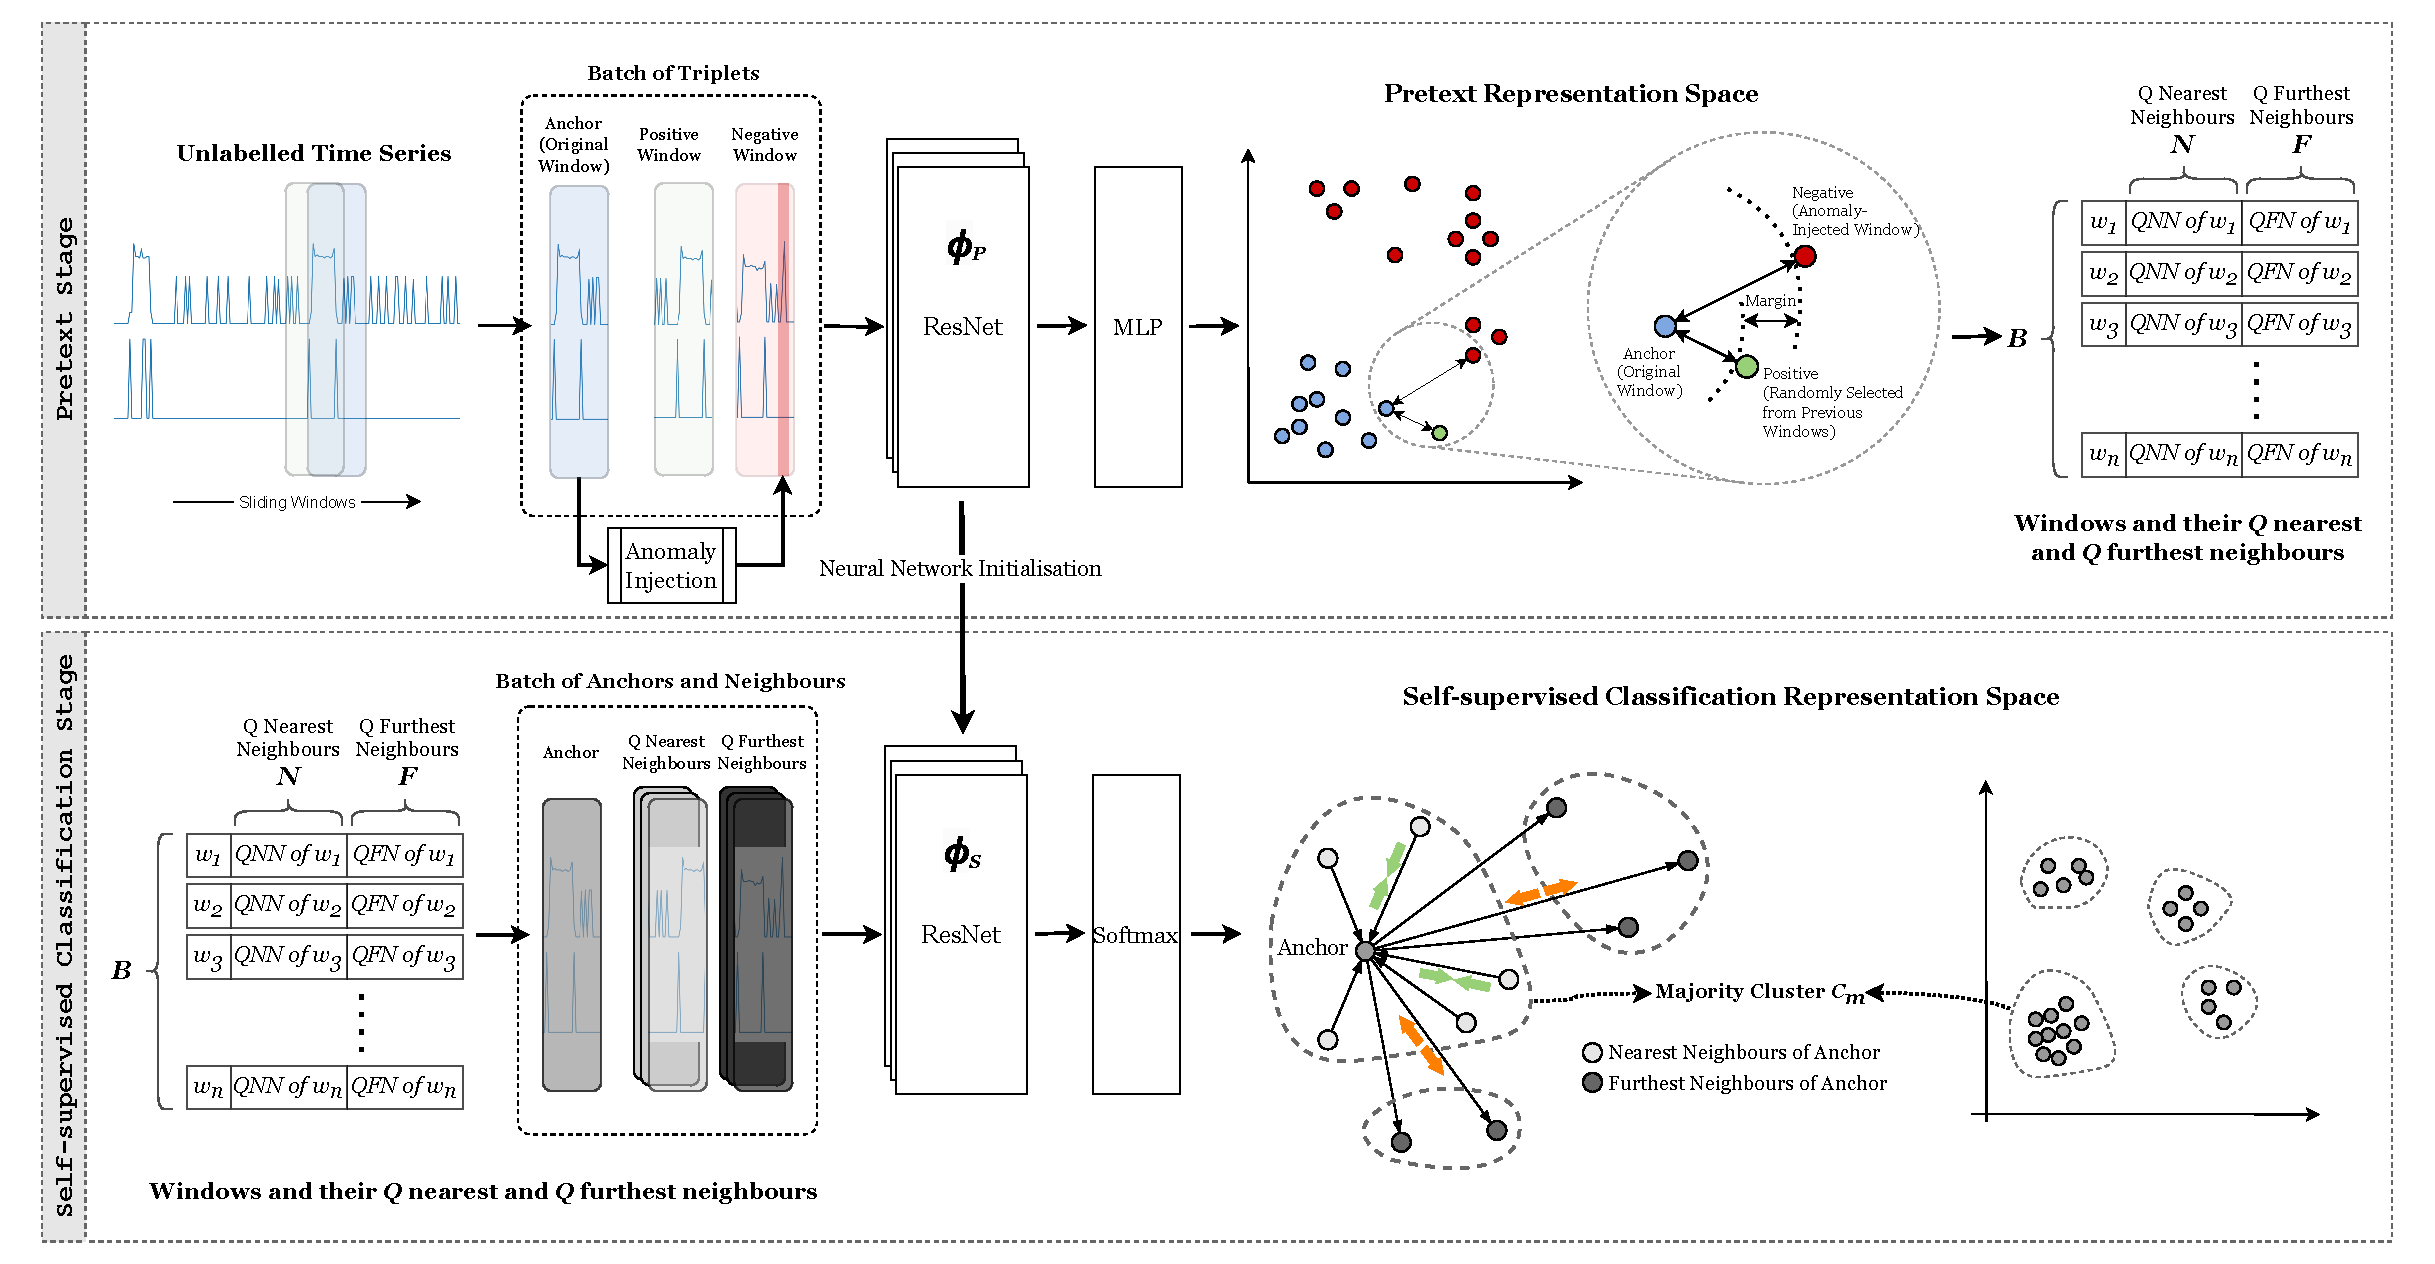
\includegraphics[
        width=1.05\linewidth,
        height=0.78\textheight,
        keepaspectratio
    ]{images/figure1_a}
    \caption{Original CARLA architecture with ResNet backbone in both stages \cite{darban2024carla}.}
    \label{fig:carla_resnet}
\end{figure}

\begin{figure}[H]
    \centering
    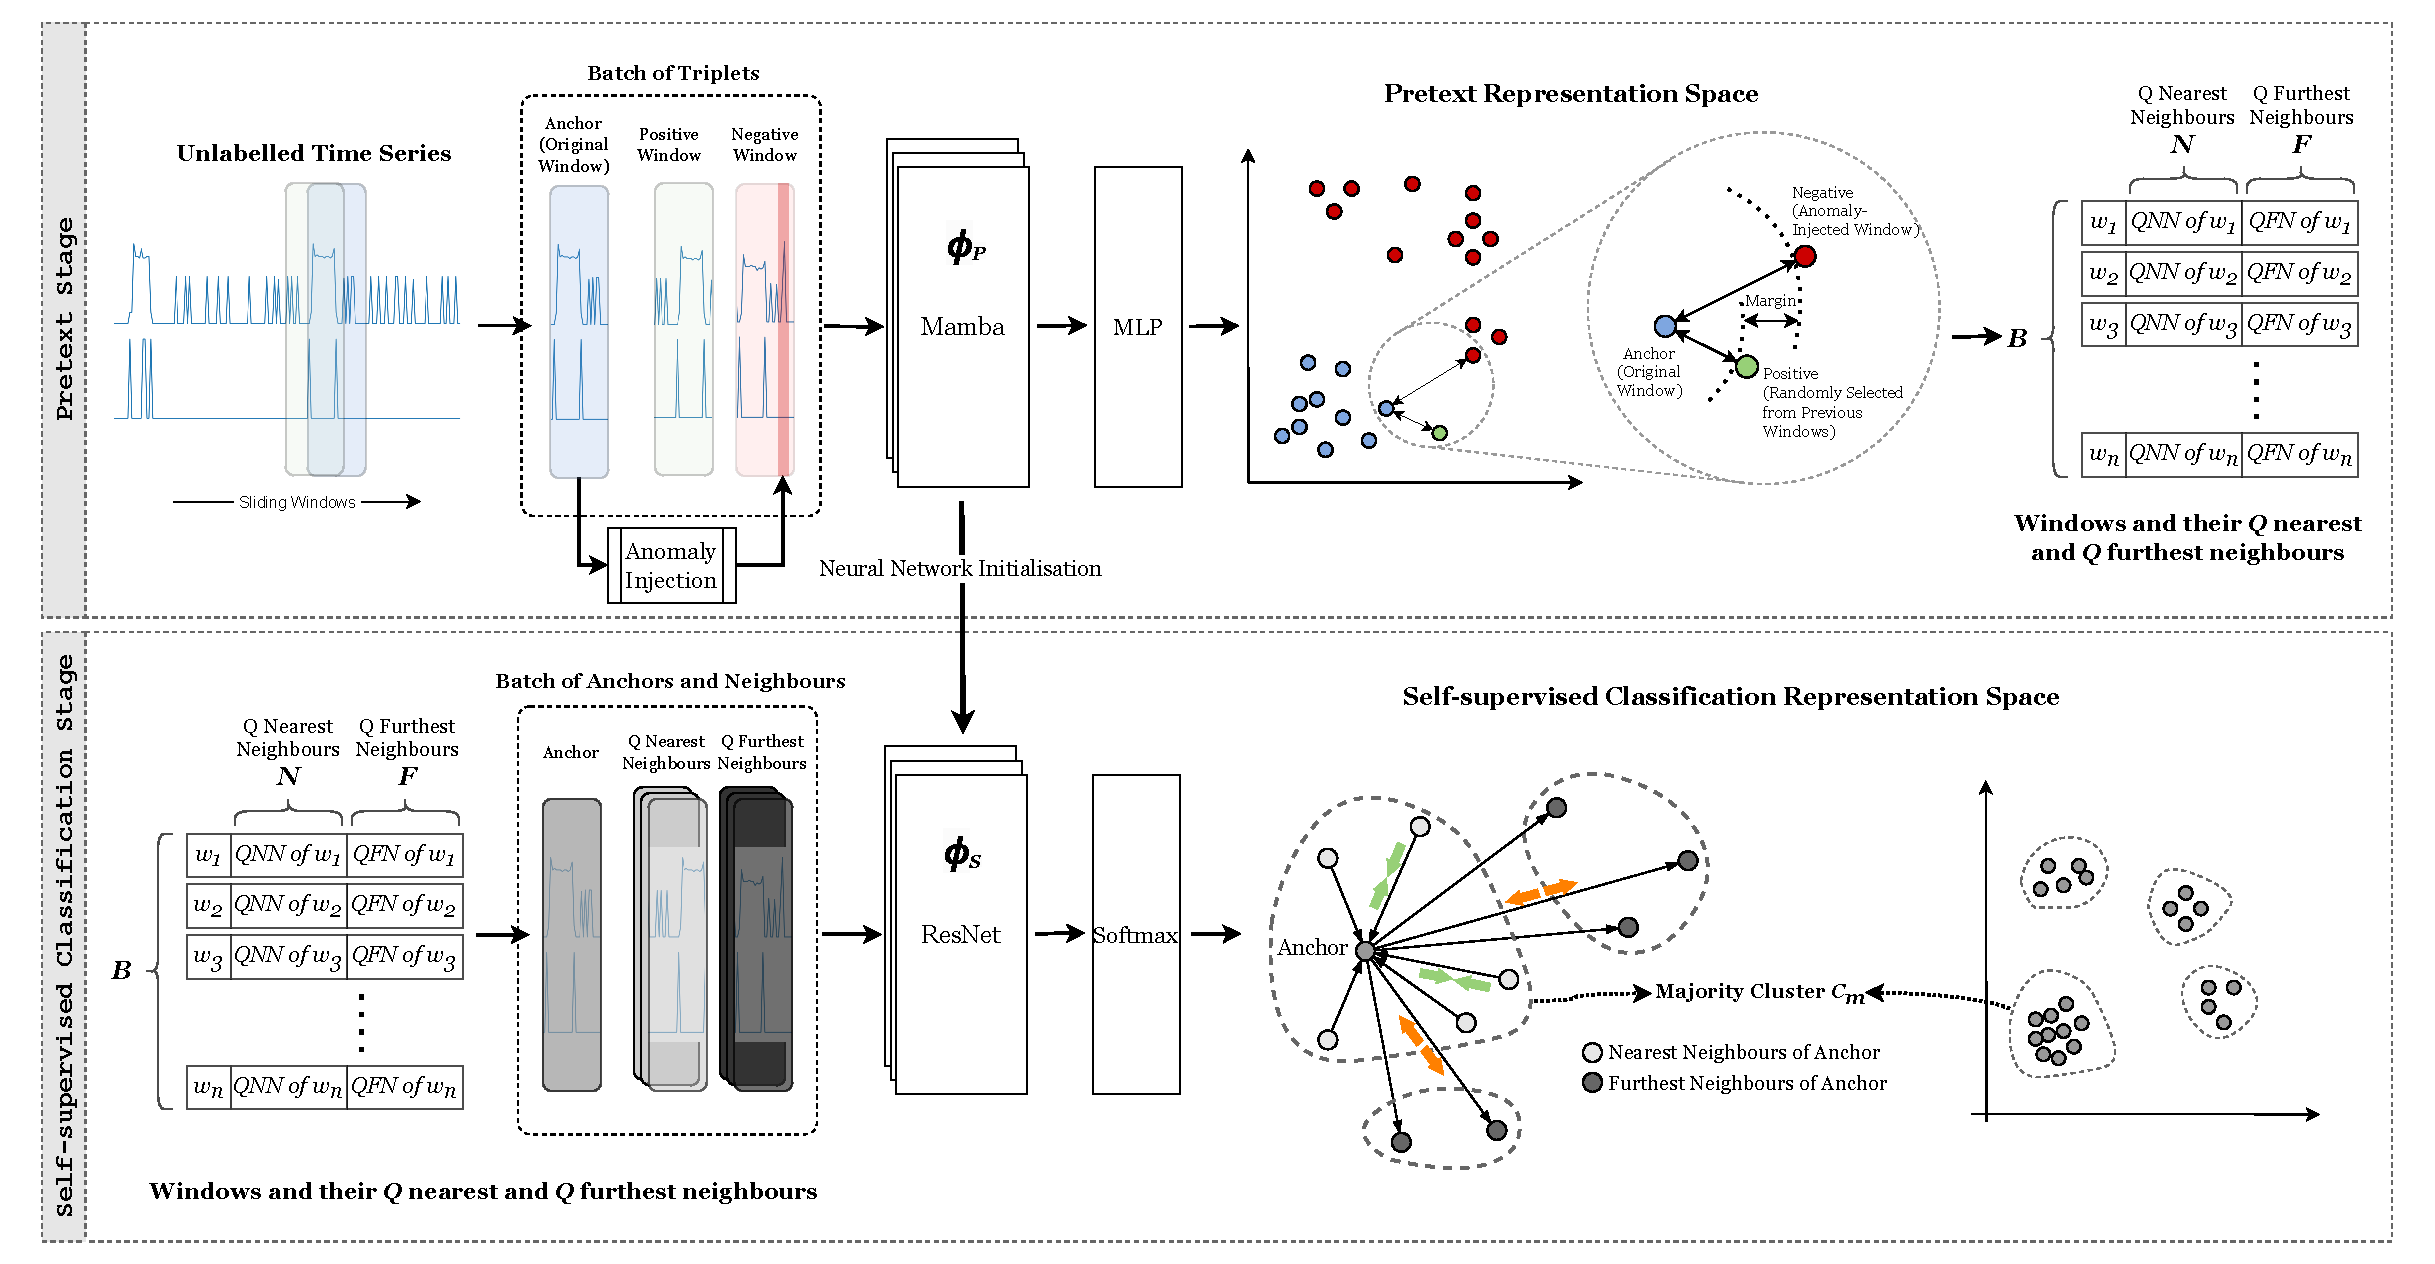
\includegraphics[
        width=1.05\linewidth,
        height=0.78\textheight,
        keepaspectratio
    ]{images/figure1_c}
    \caption{CARLA-MAMBA: Mamba replaces ResNet in the pretext stage only.}
    \label{fig:carla_mamba}
\end{figure}

\subsection{Datasets}

We evaluate our method on seven widely used benchmark datasets for time-series anomaly detection. These datasets cover diverse characteristics, including multivariate and univariate time series, different anomaly ratios, and multiple application domains such as spacecraft monitoring, industrial systems, and web services.

\begin{table}[H]
\centering
\caption{Summary of benchmark datasets used in our experiments.}
\label{tab:datasets}
\resizebox{\linewidth}{!}{
\begin{tabular}{lcccccc}
\hline
\textbf{Dataset} & \textbf{\#Series} & \textbf{Dims} & \textbf{Train Size} & \textbf{Test Size} & \textbf{Anomaly (\%)} & \textbf{Ref} \\
\hline
MSL      & 27 & 55  & 58,317  & 73,729  & 10.53 & \cite{msl_smap_dataset} \\
SMAP     & 55 & 25  & 140,825 & 444,035 & 12.85 & \cite{msl_smap_dataset} \\
SMD      & 28 & 38  & 708,405 & 708,420 & 4.16  & \cite{smd_dataset} \\
SWaT     & 1  & 51  & 496,800 & 449,919 & 12.14 & \cite{swat_dataset_kaggle} \\
WADI     & 1  & 123 & 784,568 & 172,801 & 5.77  & \cite{wadi_dataset_kaggle} \\
Yahoo-A1 & 55 & 1   & 39,096  & 39,136  & 3.79  & \cite{yahoo_a1_dataset} \\
KPI      & 29 & 1   & 1,459,418 & 1,459,429 & 2.21 & \cite{kpi_dataset} \\
\hline
\end{tabular}
}
\end{table}

All datasets are publicly available and have been widely used in prior research. The train/test splits follow the original CARLA protocol, and no additional preprocessing is applied.

\subsection{Training Protocol}

To ensure a fair and reproducible comparison, all experiments are conducted on a single NVIDIA Tesla T4 GPU with 16~GB of memory. Both CARLA-ResNet and CARLA-MAMBA are independently tuned to achieve the best possible performance for their respective backbone architectures. The backbone architecture and the window size are tuned separately for each variant, while other hyperparameters such as learning rate, batch size, number of epochs, and optimizer are kept the same for each dataset.

For CARLA-ResNet, we follow the original CARLA implementation \cite{darban2024carla} and use the window sizes selected by the original authors: 200 for MSL, SMAP, SMD, and SWaT; 400 for WADI; and 250 for Yahoo-A1 and KPI. These values were reported as optimal for the ResNet backbone by the original authors.

For CARLA-MAMBA, we use window sizes that are powers of two, which are better suited for the Mamba architecture: 256 for MSL, SMAP, SMD, and SWaT; and 512 for Yahoo-A1 and KPI.

For training epochs, SWaT and WADI use 10 pretext epochs while the other datasets use 30. This is because SWaT and WADI are large single-series datasets that require more time per epoch, and the T4 GPU session time is limited. The same number of epochs is used for both variants on each dataset.

Table~\ref{tab:hyperparams} summarizes the key hyperparameters.

\begin{table}[H]
\centering
\caption{Hyperparameter settings for CARLA-ResNet and CARLA-MAMBA. Each variant is independently tuned for its backbone. Window sizes differ between the two variants.}
\label{tab:hyperparams}
\resizebox{\linewidth}{!}{
\begin{tabular}{lcc}
\hline
\textbf{Parameter} & \textbf{CARLA-ResNet} & \textbf{CARLA-MAMBA} \\
\hline
Backbone (pretext) & ResNet (3 layers, kernels $[8,5,3]$) & Mamba (3 layers, $d\_state{=}16$, $d\_conv{=}4$, $expand{=}2$) \\
Backbone (classification) & ResNet & ResNet \\
Window size (MSL, SMAP, SMD, SWaT) & 200 & 256 \\
Window size (WADI) & 400 & 256 \\
Window size (Yahoo-A1, KPI) & 250 & 512 \\
Epochs (pretext) & 30 (10 for SWaT/WADI) & 30 (10 for SWaT/WADI) \\
Epochs (classification) & 50 & 50 \\
Learning rate (pretext) & 0.001 & 0.001 \\
Batch size & 50 (64--256 for SWaT/WADI) & 50 (64--256 for SWaT/WADI) \\
Optimizer & Adam & Adam \\
\hline
\end{tabular}
}
\end{table}

\subsection{Evaluation Metrics}

We evaluate using Precision, Recall, F1-score, and AU-PR. We do not use Point Adjustment (PA) because it can lead to an overestimation of performance \cite{kim2022towards}. We also measure total inference time, average inference time per file, and peak GPU memory usage.

% ---- Results ----
\section{Results}
\label{sec:results}

This section presents the experimental results of CARLA-ResNet and CARLA-MAMBA on seven benchmark datasets. All experiments are conducted on a single Tesla T4 GPU.

\begin{figure}[t]
    \centering
    
    \begin{subfigure}[t]{0.48\linewidth}
        \centering
        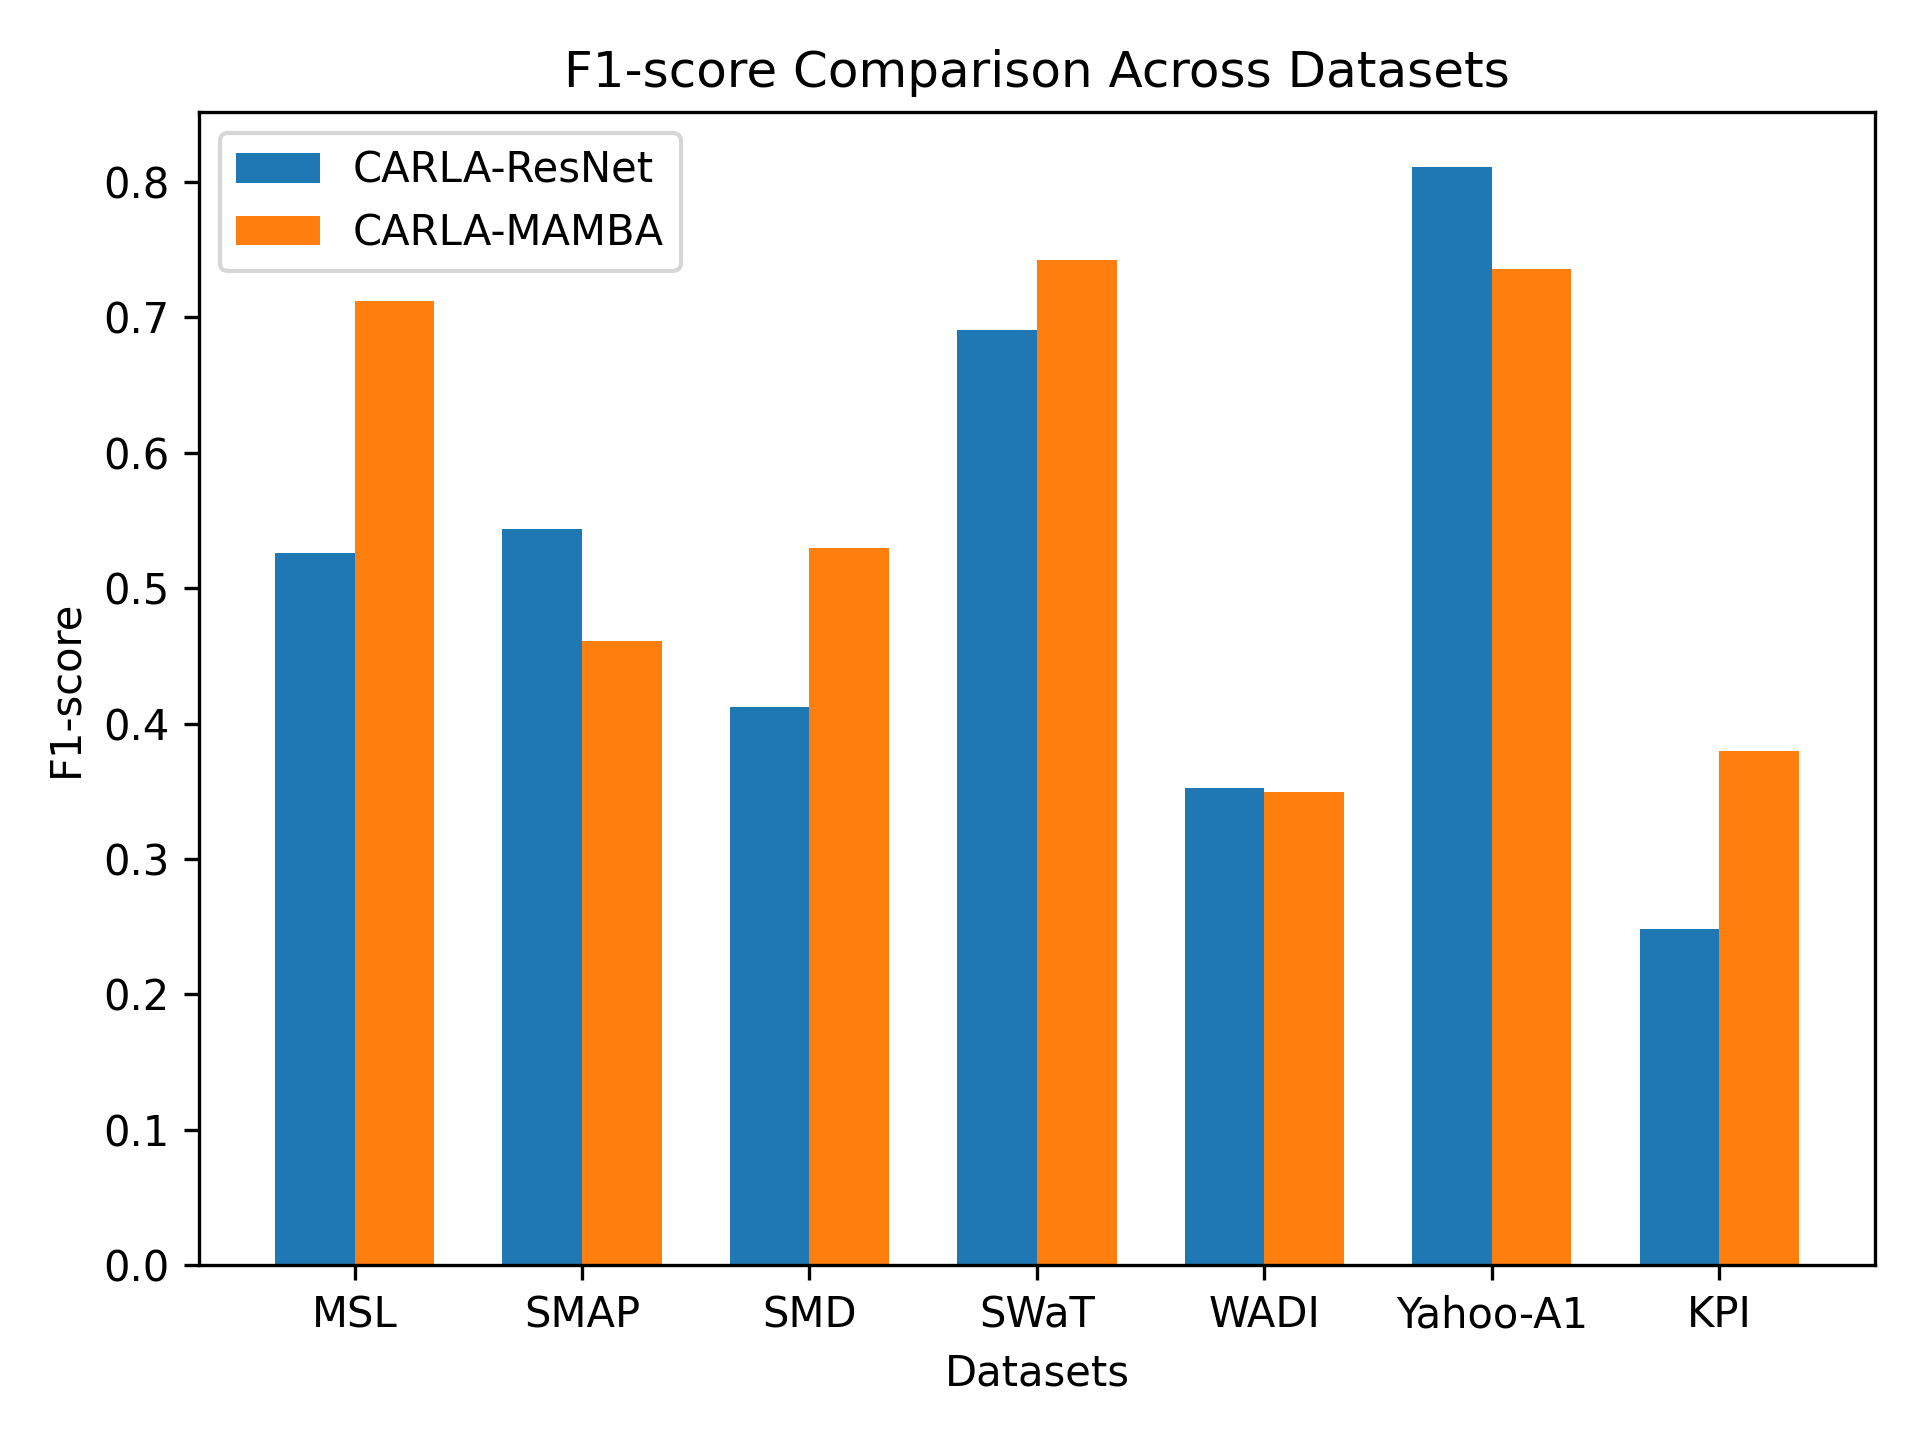
\includegraphics[width=\linewidth]{images/f1_comparison.png}
        \caption{F1-score comparison}
        \label{fig:f1_comparison}
    \end{subfigure}
    \hfill
    \begin{subfigure}[t]{0.48\linewidth}
        \centering
        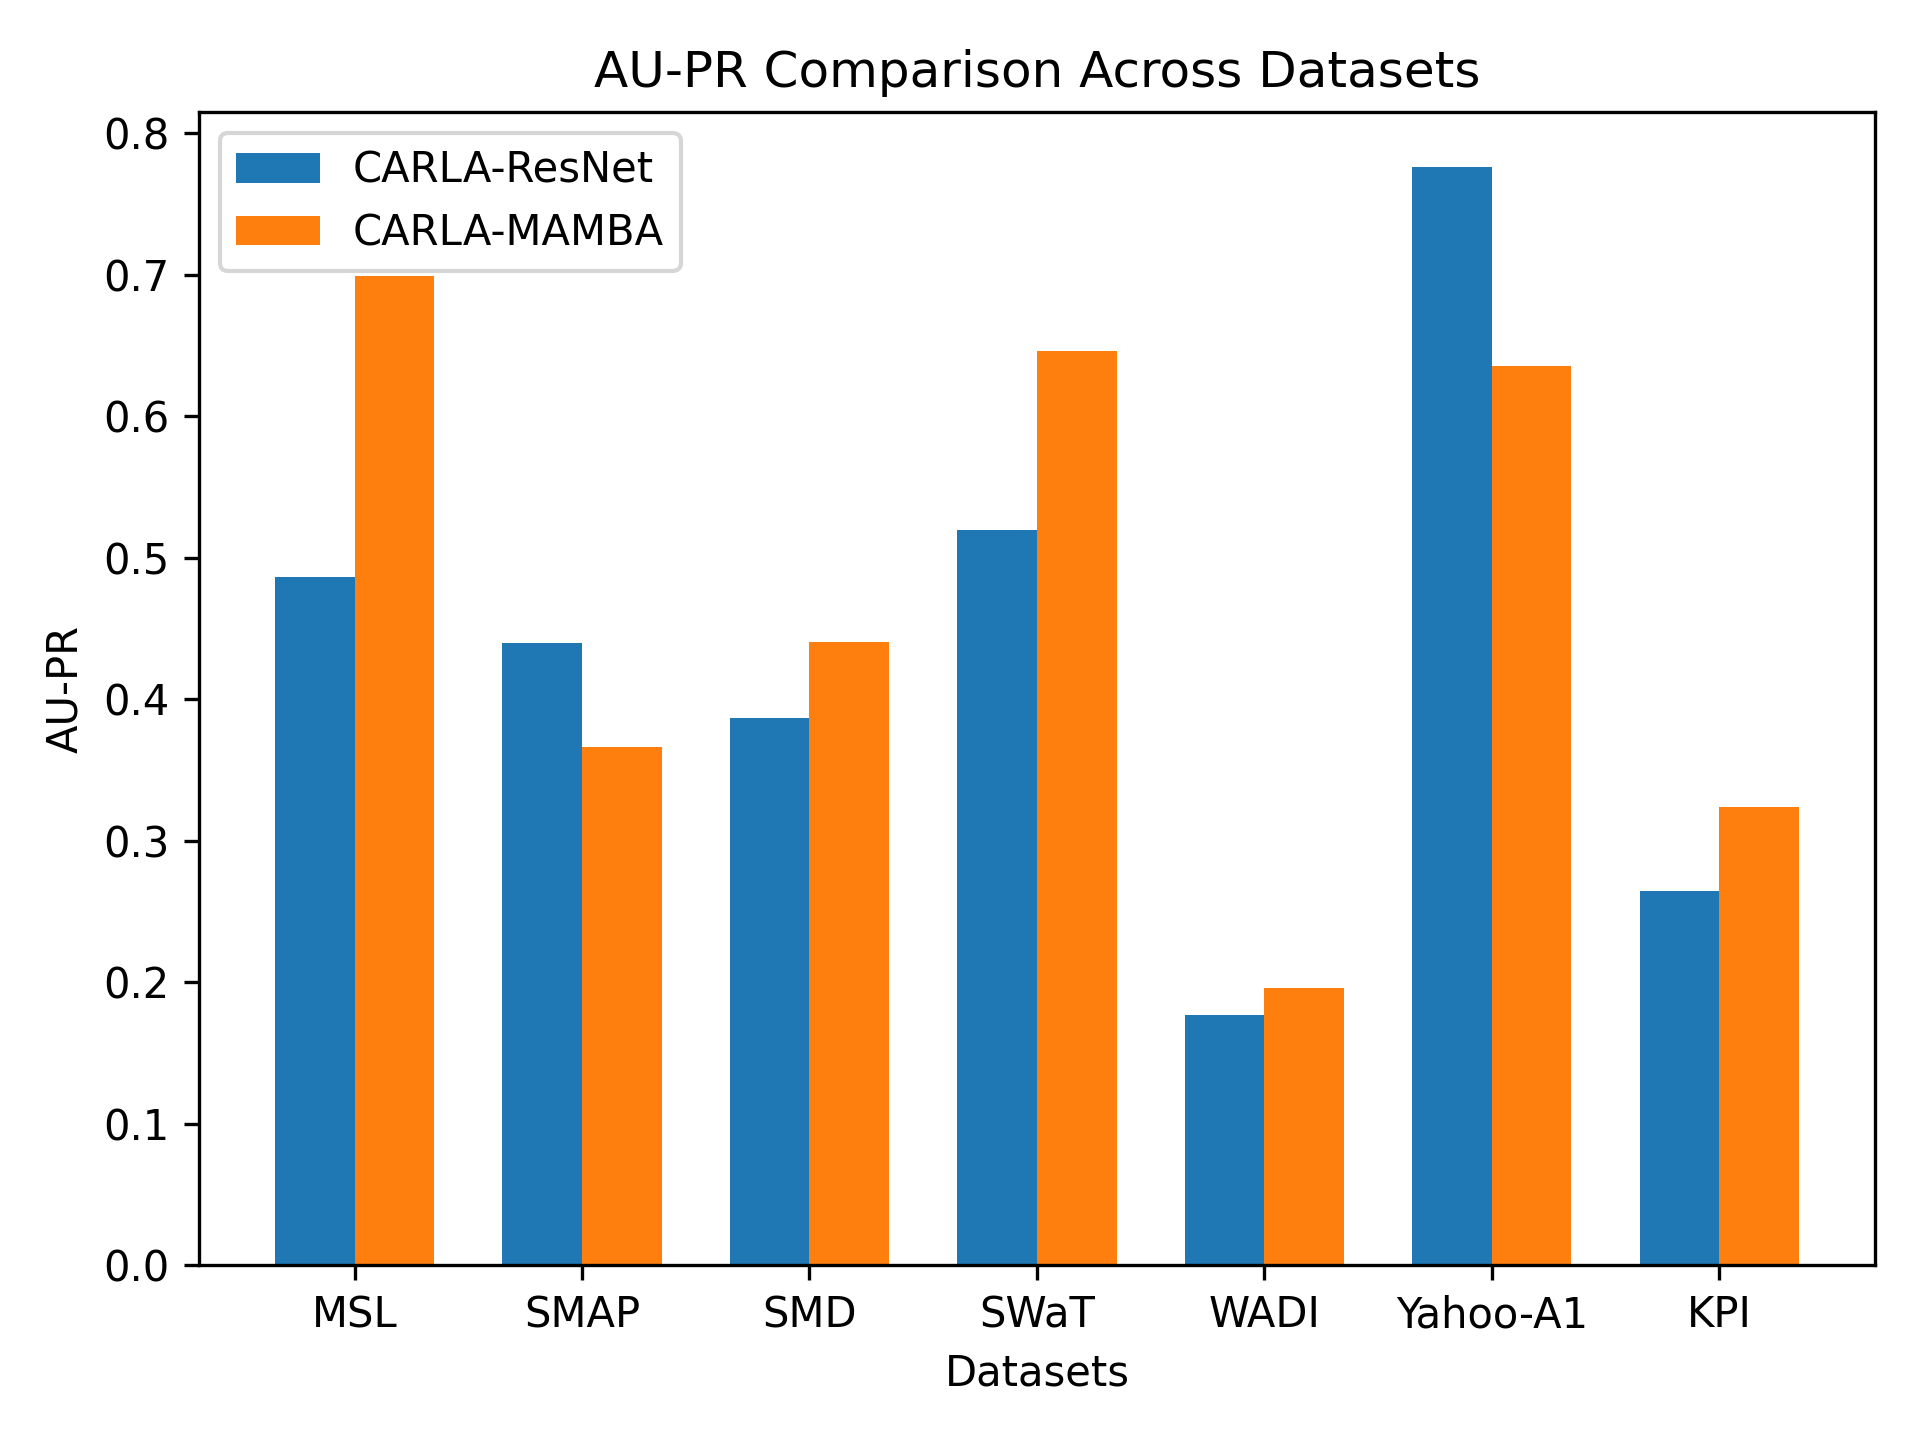
\includegraphics[width=\linewidth]{images/aupr_comparison.png}
        \caption{AU-PR comparison}
        \label{fig:aupr_comparison}
    \end{subfigure}
    
    \caption{Comparison of CARLA-ResNet and CARLA-MAMBA across seven benchmark datasets in terms of F1-score and AU-PR.}
    \label{fig:combined_results}
\end{figure}

Figure~\ref{fig:combined_results} presents the comparison between CARLA-ResNet and CARLA-MAMBA across all datasets. 
CARLA-MAMBA outperforms the ResNet baseline on most datasets, particularly on MSL, SMD, SWaT, and KPI. 
It also achieves higher AU-PR on MSL, SMD, SWaT, WADI, and KPI, indicating better ranking performance for anomaly detection.

\subsection{Overall Performance}

Table~\ref{tab:carla_comparison} shows the results of both variants. CARLA-MAMBA achieves higher F1 and AU-PR than the ResNet baseline on four out of seven datasets: MSL, SMD, SWaT, and KPI. On MSL, F1 improves from 0.5258 to 0.7120 and AU-PR 
from 0.4866 to 0.6987. On SMD, F1 improves from 0.4123 
to 0.5300 and AU-PR from 0.3870 to 0.4401. On SWaT, 
CARLA-MAMBA achieves perfect precision (1.0000) with a 
higher F1 of 0.7427 compared to 0.6908. On KPI, F1 
improves from 0.2483 to 0.3798.

On SMAP and Yahoo-A1, CARLA-MAMBA shows lower F1 than the baseline. On WADI, the two variants perform similarly, with CARLA-MAMBA slightly lower in F1 but slightly higher in AU-PR.

\begin{table}[H]
\centering
\caption{Performance and efficiency comparison of CARLA variants on seven benchmark datasets. All experiments use a single Tesla T4 GPU.}
\label{tab:carla_comparison}
\resizebox{\linewidth}{!}{
\begin{tabular}{llccccccc}
\hline
\textbf{Dataset} & \textbf{Method} &
\textbf{Prec} & \textbf{Rec} & \textbf{F1} & \textbf{AU-PR} &
\textbf{Time (s)} & \textbf{Avg.(s)} & \textbf{Mem.(MB)} \\
\hline
\multirow{2}{*}{MSL}
 & ResNet  & 0.3910 & 0.8025 & 0.5258 & 0.4866 $\pm$ 0.2519 & 12351.98 & 457.48 & 1230.80 \\
 & MAMBA   & \textbf{0.6132} & \textbf{0.8487} & \textbf{0.7120} & \textbf{0.6987 $\pm$ 0.1693} & 10789.86 & 399.62 & 2884.31 \\
\hline
\multirow{2}{*}{SMAP}
 & ResNet  & \textbf{0.4233} & 0.7589 & \textbf{0.5435} & \textbf{0.4396 $\pm$ 0.3217} & 33924.34 & 616.81 & 382.69 \\
 & MAMBA   & 0.3189 & \textbf{0.8322} & 0.4611 & 0.3663 $\pm$ 0.3137 & 30623.82 & 556.80 & 469.62 \\
\hline
\multirow{2}{*}{SMD}
 & ResNet  & 0.3144 & 0.5987 & 0.4123 & 0.3870 $\pm$ 0.1908 & 33763.76 & 1205.85 & 1540.48 \\
 & MAMBA   & \textbf{0.3884} & \textbf{0.8340} & \textbf{0.5300} & \textbf{0.4401 $\pm$ 0.1808} & 33093.38 & 1181.91 & 3840.36 \\
\hline
\multirow{2}{*}{SWaT}
 & ResNet  & 0.7917 & \textbf{0.6126} & 0.6908 & 0.5193 & 1142.35 & 1142.35 & 206.96 \\
 & MAMBA   & \textbf{1.0000} & 0.5907 & \textbf{0.7427} & \textbf{0.6457} & 1124.73 & 1124.73 & 467.78 \\
\hline
\multirow{2}{*}{WADI}
 & ResNet  & 0.2202 & \textbf{0.8824} & \textbf{0.3525} & 0.1771 & 1496.77 & 1496.77 & 179.48 \\
 & MAMBA   & \textbf{0.2298} & 0.7314 & 0.3497 & \textbf{0.1959} & 1433.61 & 1433.61 & 297.37 \\
\hline
\multirow{2}{*}{Yahoo-A1}
 & ResNet  & \textbf{0.6946} & 0.9746 & \textbf{0.8111} & \textbf{0.7761 $\pm$ 0.3397} & 5609.75 & 102.00 & 42.39 \\
 & MAMBA   & 0.5864 & \textbf{0.9867} & 0.7356 & 0.6355 $\pm$ 0.3941 & 5845.12 & 106.27 & 92.93 \\
\hline
\multirow{2}{*}{KPI}
 & ResNet  & 0.1500 & 0.7206 & 0.2483 & 0.2644 $\pm$ 0.2343 & 62356.69 & 2150.23 & 371.06 \\
 & MAMBA   & \textbf{0.2453} & \textbf{0.8415} & \textbf{0.3798} & \textbf{0.3235 $\pm$ 0.2276} & 66186.61 & 2282.30 & 316.46 \\
\hline
\end{tabular}
}
\end{table}

\subsection{Inference Time and Memory}

In terms of inference time, CARLA-MAMBA is slightly faster than the ResNet baseline on most datasets (e.g., MSL, SMAP, SMD, SWaT, WADI). This is because Mamba uses a parallel scan algorithm that avoids the sequential bottleneck of recurrent models \cite{gu2023mamba}. On Yahoo-A1 and KPI, the inference time is slightly higher for CARLA-MAMBA, but the difference is small.

Regarding GPU memory, CARLA-MAMBA uses more memory than the baseline on datasets with more dimensions (MSL, SMD, SWaT, WADI). This is because Mamba maintains a larger internal state. On Yahoo-A1 and KPI, which are univariate datasets, the memory difference is smaller.

% ---- Discussion ----
\section{Discussion}

\subsection{Where Mamba Helps and Why}

Our experiments show that replacing the ResNet backbone with Mamba in the pretext stage improves anomaly detection on four of seven datasets: MSL, SMD, SWaT, and KPI. We believe the main reason is that Mamba can model temporal dependencies beyond the local range of ResNet's convolutional kernels ($[8, 5, 3]$). On these datasets, Mamba's selective state space mechanism helps the pretext encoder build richer representations that better separate normal and anomalous patterns.

The improvement is especially large on MSL (F1: $0.5258 \to 0.7120$, $+35.4\%$) and KPI (F1: $0.2483 \to 0.3798$, $+52.9\%$). On both datasets, CARLA-MAMBA improves both precision and recall at the same time, which means the learned representations create better-separated groups in the embedding space. This leads to more accurate neighbor assignments for the classification stage.

On SWaT, Mamba achieves perfect precision ($1.0000$), which means every window it marks as anomalous is truly anomalous. However, the recall is slightly lower ($0.5907$ vs.\ $0.6126$). This suggests that Mamba-based representations produce a more careful but very reliable decision boundary.

\subsection{Where Mamba Falls Short: Precision--Recall Analysis}

On SMAP and Yahoo-A1, CARLA-MAMBA achieves lower F1-scores than the ResNet baseline. A closer look at the results shows a clear pattern in the precision--recall trade-off.

\textbf{Higher recall but much lower precision.} On both datasets, Mamba achieves \emph{higher recall} than ResNet (SMAP: $0.8322$ vs.\ $0.7589$; Yahoo-A1: $0.9867$ vs.\ $0.9746$) but \emph{much lower precision} (SMAP: $0.3189$ vs.\ $0.4233$; Yahoo-A1: $0.5864$ vs.\ $0.6946$). This means Mamba detects more true anomalies but also produces many more false positives. The precision drop is larger than the recall gain, which causes a lower F1-score overall.

We believe this pattern happens for several reasons. First, both SMAP and Yahoo-A1 contain many individual time series that are each quite short. Yahoo-A1 has 55 series with an average of about 710 data points per series in the training set, and SMAP has 55 series averaging about 2{,}560 training points per series. In contrast, KPI---which is also univariate but where Mamba works well---has 29 series averaging over 50{,}000 points each. When each series is short, there is not enough temporal context for Mamba's selective state to build useful long-range information. The model may learn false patterns within short windows, which makes the representations too sensitive and causes more normal windows to be classified as anomalous.

Second, the type of anomalies in these datasets plays an important role. The anomalies in SMAP are mostly point anomalies and short contextual anomalies \cite{hundman2018detecting}, which can be detected well by looking at local patterns. ResNet's convolutional kernels are well suited for this because the important features are within a few time steps. Mamba's global modeling may add unwanted noise when the anomaly signal is already local.

Third, Mamba's state space mechanism processes the full sequence with a continuous transformation. When anomalies are short and local, this global processing can reduce the anomaly signal in the learned representation---an effect similar to over-smoothing. This makes it harder for the classification stage to separate anomalous windows from normal ones, which explains the lower precision.

\subsection{The WADI Case}

On WADI, the two variants perform almost the same (F1: $0.3525$ vs.\ $0.3497$), with CARLA-MAMBA achieving slightly higher AU-PR ($0.1959$ vs.\ $0.1771$). WADI is a difficult dataset for all methods because it has very high dimensionality (123 features), a low anomaly ratio ($5.77\%$), and complex dependencies between sensors in an industrial water treatment system. Both ResNet and Mamba achieve low precision (about $0.22$), which shows that the difficulty is not in the backbone but in the classification and threshold selection steps. The small AU-PR improvement suggests that Mamba does produce slightly better-ranked anomaly scores, even though the final binary classification results are nearly the same.

\subsection{Limitations}

This work has several limitations. First, CARLA-MAMBA uses more GPU memory than the ResNet baseline on high-dimensional datasets (for example, $2{,}884$~MB vs.\ $1{,}231$~MB on MSL), which may be a problem on hardware with limited memory. Second, only the pretext stage backbone is replaced with Mamba. We also tested using Mamba in the classification stage, but the results were worse than using ResNet, so this approach was not adopted. Third, our experiments use a single run with a fixed random seed. Adding results from multiple random seeds would make the comparison more reliable.

\subsection{Future Work}

Several directions could be explored in future work. First, a per-series analysis on multi-series datasets like SMAP (55 series) could show which types of series benefit most from long-range modeling and provide deeper insight into when Mamba is most effective. Second, combining Mamba with attention mechanisms may help balance local and global feature learning, which could improve performance on datasets where local anomalies are dominant, such as SMAP and Yahoo-A1. Third, applying CARLA-MAMBA to other application domains such as healthcare monitoring or financial fraud detection could test whether the benefits of Mamba generalize beyond the benchmark datasets used in this study. Finally, exploring other recent state space model variants beyond Mamba, such as Mamba-2 or other selective SSM architectures, may further improve the quality of learned representations in the pretext stage.

% ---- Conclusion ----
\section{Conclusion}

In this paper, we proposed CARLA-MAMBA, a variant of the CARLA framework for time-series anomaly detection. We replaced the ResNet backbone in the pretext stage with Mamba, a selective state space model that is better suited for sequential data. The classification stage still uses ResNet, but it benefits from improved neighbor sets computed using the Mamba embeddings.

We tested our method on seven benchmark datasets. CARLA-MAMBA outperforms the original CARLA baseline on four datasets (MSL, SMD, SWaT, KPI) in terms of both F1-score and AU-PR. On two datasets (SMAP, Yahoo-A1), the baseline performs better due to a systematic precision drop caused by the interaction between Mamba's global modeling and the short, local nature of the anomalies. On WADI, both variants perform similarly.

Our results show that the backbone choice in the pretext stage has a meaningful effect on anomaly detection performance. Mamba is a promising backbone for datasets with long sequences and complex temporal patterns. For datasets with short sequences and local anomalies, simpler architectures like ResNet may be more suitable. Future work will explore combining Mamba with attention mechanisms and applying the method to other application domains.

% ---- Bibliography ----
\bibliographystyle{splncs03_unsrt}
\bibliography{references}

\end{document}